\documentclass[a4paper,10pt]{report}

\topmargin -2cm
%\topskip0cm
%\footskip0cm
%\headsep0cm
\parindent0cm
\oddsidemargin -1cm
\evensidemargin -1cm
\headheight 2cm
\textheight 24cm
\textwidth 18cm

\author{Alexander M\"unn (4403061)}
\title{\"Ubung}

\usepackage{ucs}
\usepackage[utf8x]{inputenc}
\usepackage{german}
\usepackage{color}
\usepackage{url}
\usepackage{graphicx}
\usepackage{algorithmic}

\pagestyle{empty}
\usepackage{float}
\usepackage{makeidx}
\usepackage{amsmath}
\usepackage{amsfonts}
\usepackage{amssymb,euscript}
\usepackage{dsfont}
\usepackage{listings}
\usepackage{enumerate}
\newfont{\Fr}{eufm10}
\newfont{\Sc}{eusm10}
\newfont{\Bb}{msbm10}
\newcommand{\limin}{\lim_{n\rightarrow\infty}}
\newcommand{\limix}{\lim_{x\rightarrow\infty}}
\newcommand{\limun}{\lim_{n\rightarrow -\infty}}
\newcommand{\limux}{\lim_{n\rightarrow -\infty}}
\newcommand{\limx}{\lim_{x\rightarrow x_0}}
\newcommand{\limh}{\lim_{h\rightarrow 0}}
\newcommand{\defi}{\paragraph{Definition:}}
\newcommand{\bew}{\paragraph{Beweis:}}
\newcommand{\satz}{\paragraph{Satz:}}
\newcommand{\bsp}{\paragraph{Beispiel:}}
\newcommand{\lemma}{\paragraph{Lemma:}}
\newcommand{\N}{\mathds{N}}
\newcommand{\F}{\mathds{F}}
\newcommand{\Z}{\mathds{Z}}
\newcommand{\Q}{\mathds{Q}}
\newcommand{\R}{\mathds{R}}
\newcommand{\G}{\mathds{G}}
\newcommand{\C}{\mathds{C}}
\newcommand{\K}{\mathds{K}}
\newcommand{\A}{\mathds{A}}
\newcommand{\E}{\mathcal{E}}
\renewcommand{\P}{\mathcal{P}}
\newcommand{\sigA}{$\sigma$-Algebra }
\newcommand{\qed}{$\hfill\blacksquare$}
\newcommand{\arsinh}{\operatorname{arsinh} }
\newcommand{\arcosh}{\operatorname{arcosh} }
\newcommand{\gdw}{ $ \Leftrightarrow $ }
\newcommand{\tf}{ $ \Rightarrow $ }
\newcommand{\mgdw}{\Leftrightarrow}
\newcommand{\mtf}{\Rightarrow}
\newcommand{\Bild}{\text{Bild}}
\newcommand{\Kern}{\text{kern}}
\newcommand{\rg}{\text{rg}}
\newcommand{\deff}{\text{deff}}

\newcommand{\alphato}{\underset{\alpha}\to}
\newcommand{\betato}{\underset{\beta}\to}
\newcommand{\etato}{\underset{\eta}\to}
\newcommand{\ito}{\underset{i}\to}
\newcommand{\sto}{\underset{s}\to}
\newcommand{\kto}{\underset{k}\to}
\newcommand{\xto}{\underset{x}\to}

\usepackage{fancyhdr}
\pagestyle{fancy}
\lhead{Michael Borst\\ Alex Muenn}
\chead{"Ubungsblatt \nr\\\today}
\rhead{Computer Vision}



\newcommand{\nr}{3}

\begin{document}
\section*{Aufgabe 5}

\begin{figure}[htpb]
\begin{center}
{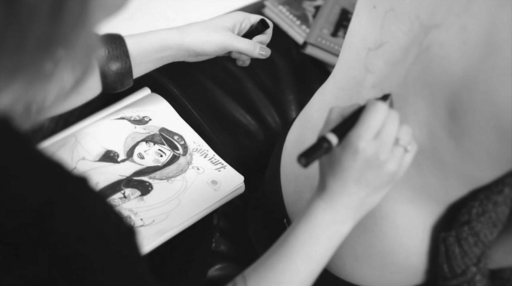
\includegraphics[width=0.25\textwidth]{samples/mrs.easy/101.png}}
{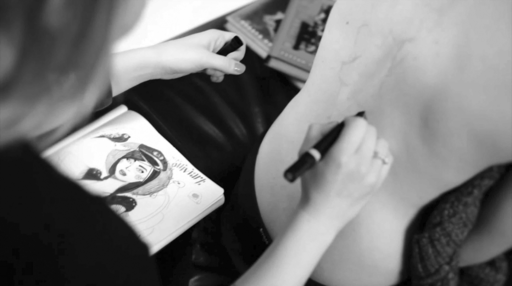
\includegraphics[width=0.25\textwidth]{samples/mrs.easy/102.png}}
\end{center}
\caption{Die Eingabebilder für die Lucas-Kanade-Berechnung }
\label{fig:u03-picture}
\end{figure}

Mit Ausführen der Datei u03.m kann Lucas-Kanade und die Vektor-Zeichnung ausgeführt werden.
Folgende Funktion errechnet die Bewegung nach Lucas-Kanade.

\lstset{language=matlab}
\begin{lstlisting}[caption={Berechnung Lucas-Kanade}]
# apply Lucas-Kanade algorithm on
# Ic - current image
# In - next image
# 
function F = lucaskanade(Ic, In, Xstep, Ystep, N)

  [rows, cols] = size(Ic);
  # calculate the gradients, r for rows, c for columns
  [Dr, Dc] = gradient(Ic);
  # calculate the general intenstiy change in the image
  Dt = Ic - In;

  F = zeros(rows,cols,2);
  # gaussian weights
  W = diag(vec(gaussmatrix(2*N+1, N)));

  for r=(1+N):(rows-N)
    for c=(1+N):(cols-N)
      # get the parameters for the l-k formula
      Ir = vec( Dr(r-N:r+N, c-N:c+N));
      Ic = vec( Dc(r-N:r+N, c-N:c+N));
      It = vec(-Dt(r-N:r+N, c-N:c+N));
      S  = [Ir Ic];
      # use pseudo-inverse to calculate vectors
      v = pinv(double(S.')*W*double(S))*double(S.')*W*double(It);
      F (r,c,:) = v;
    end
  end
end
\end{lstlisting}

Die Vektoren werden folgendermaßen erzeugt:

\lstset{language=matlab}
\begin{lstlisting}[caption={Zeichnen der Vektoren}]
# display Vectors on a picture
# Im - image
# V - vectors
# Xstep, Ystep - distance between vectors
# 
function F = drawVectorsOnImage(Im, V, Xstep, Ystep)
  [rows, cols] = size(Im);
  r = Ystep:Ystep:rows;  
  c=Xstep:Xstep:cols;
  imshow(Im);
  hold on;
  quiver(c,r,V(r,c,1),V(r,c,2),s=0);
  hold off;
end
\end{lstlisting}

\section*{Aufgabe 6}

\begin{figure}[htpb]
\begin{center}
{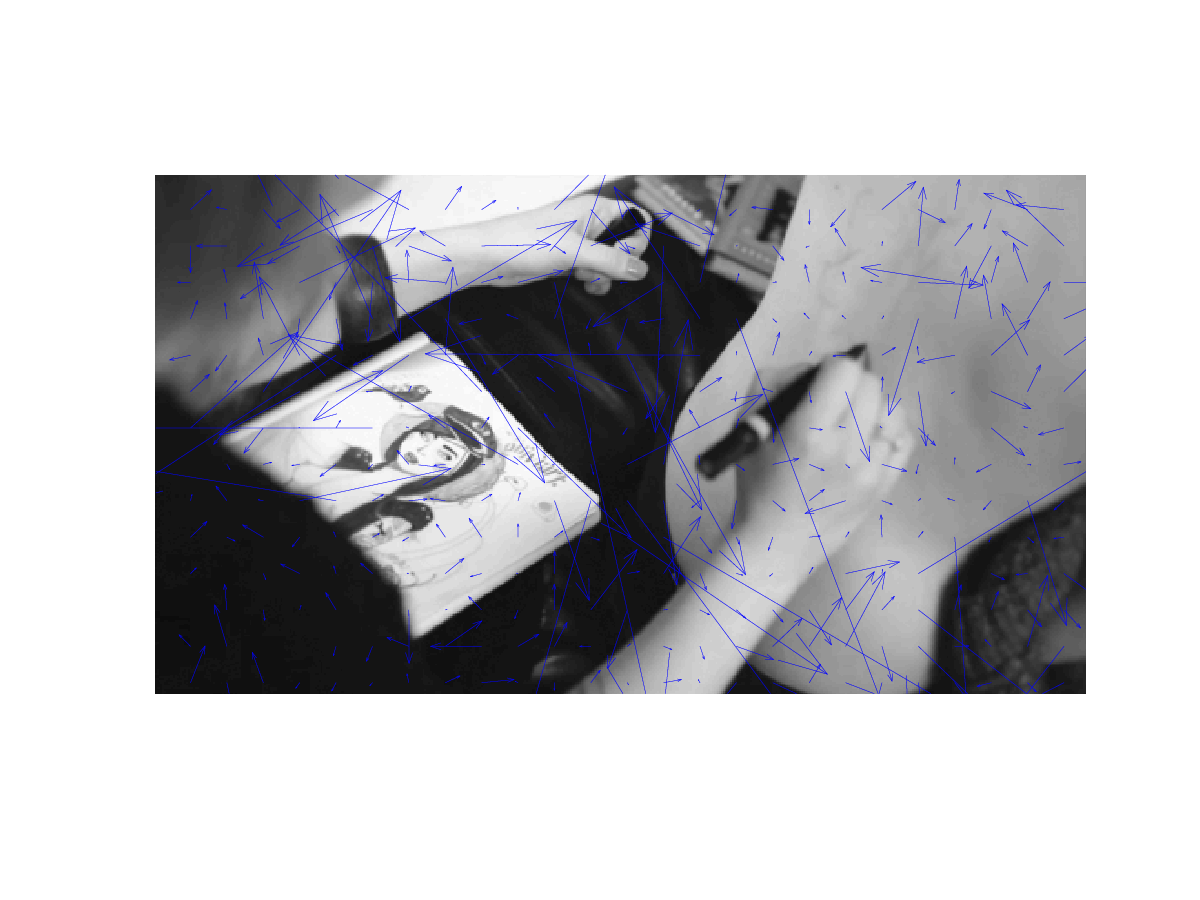
\includegraphics[width=0.45\textwidth]{u03.lucas-kanade/u03_pic_n03.png}}
{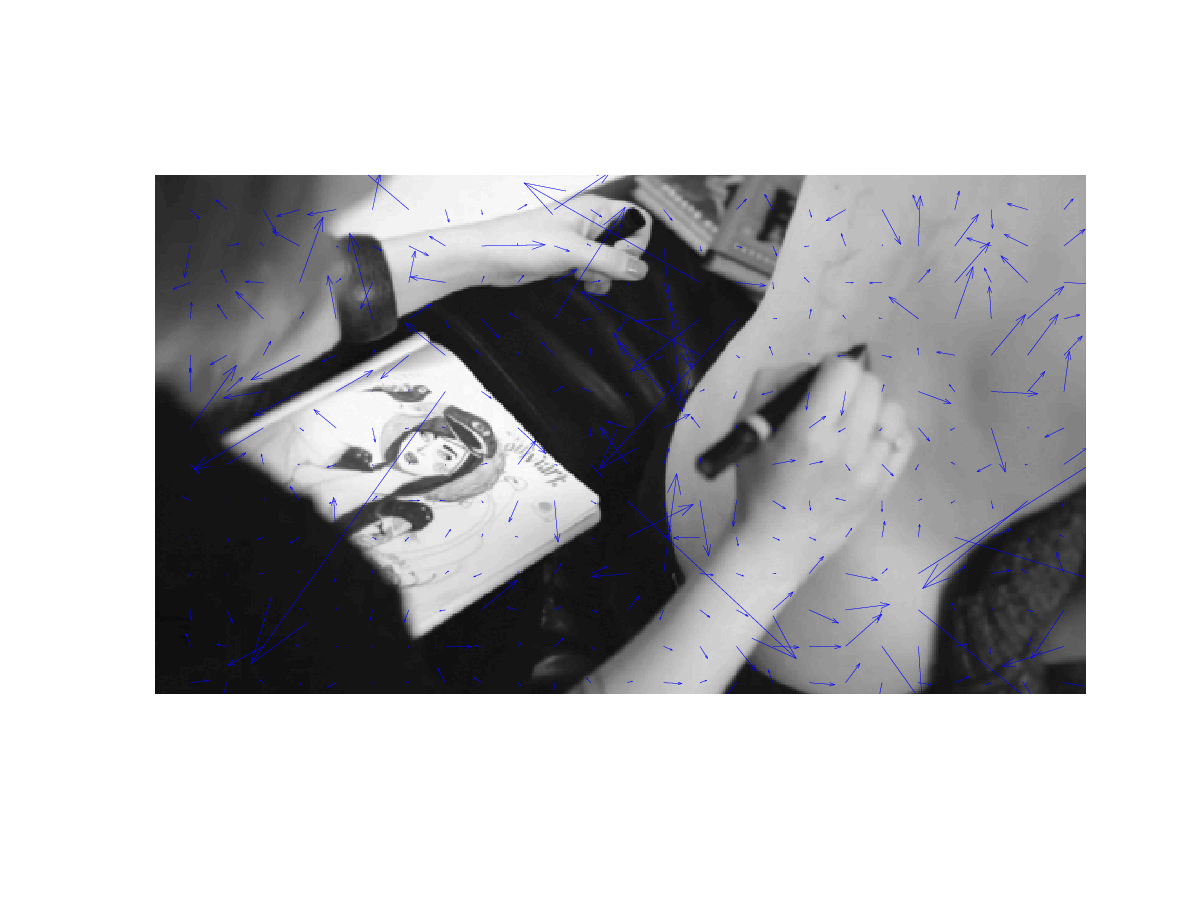
\includegraphics[width=0.45\textwidth]{u03.lucas-kanade/u03_pic_n09.png}}
{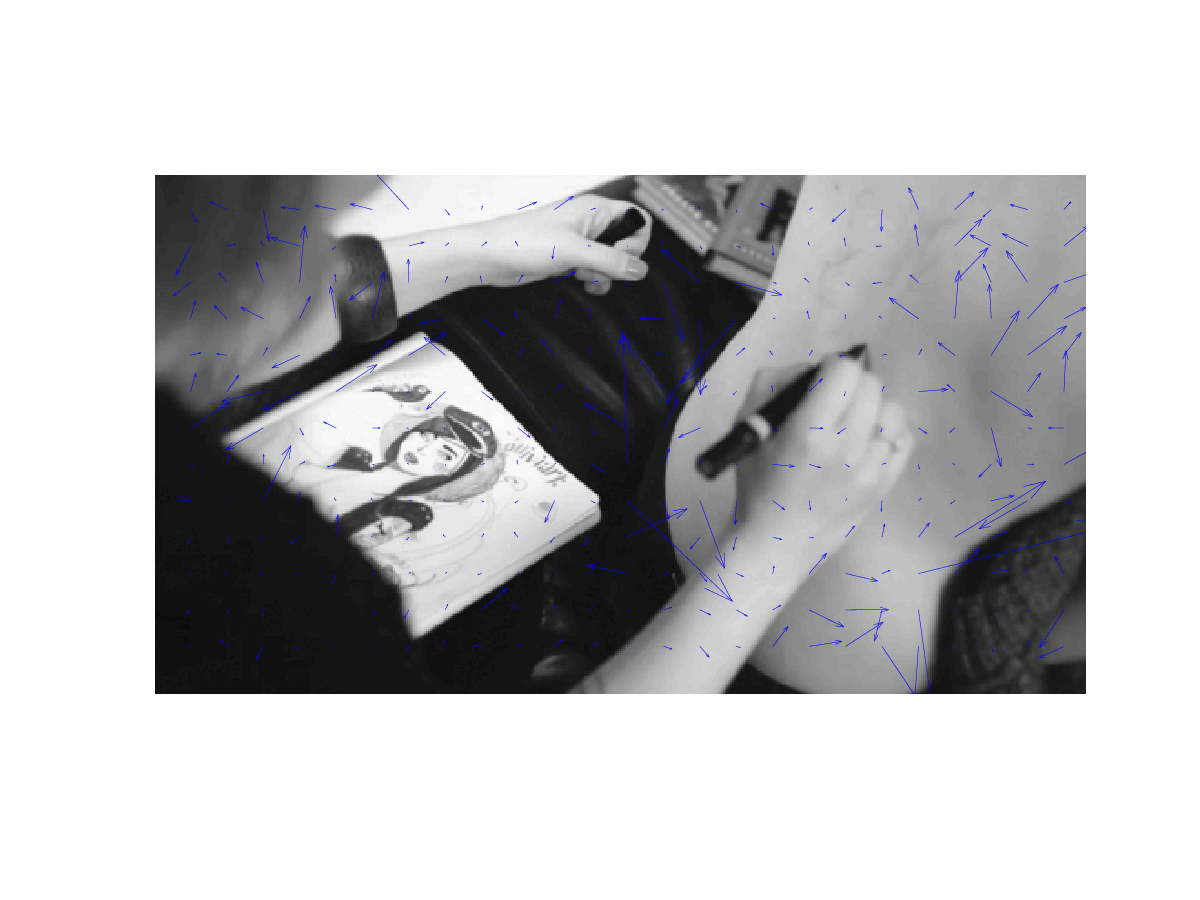
\includegraphics[width=0.45\textwidth]{u03.lucas-kanade/u03_pic_n15.png}}
\end{center}
\caption{Die Ausgabebilder für die Lucas-Kanade-Berechnung }
\label{fig:u03-t6}
\end{figure}

Wir haben für die Fenstergrößen 3x3, 9x9 und 15x15 getestet. Die Bilder finden sich auch noch in der parallel abgegebenen .zip-Datei.

% \includegraphics[width=150mm]{<file.eps>}
\end{document}
